In questo secondo esperimento si vuole studiare il comportamento di un convertitore di tensione switching - SMPC - di tipologia Buck ad \textbf{anello chiuso}. Il circuito è rappresentato in Figura \ref{fig:Circuit2}. Sono stati utilizzati i seguenti componenti:
\begin{itemize}
    \item Circuito RLC:
    \subitem Resistenza di carico $R_L=50\Omega$, ottenuta dal parallelo di due resistenze da $100\Omega,1W$
    \subitem Induttore $L=680\mu H$, come nel primo esperimento.
    \subitem Condensatore $C=20\mu F$
    \item Amplificatore operazionale 1213, codice LT1213
    \item Resistenze varie 
    \item Condensatori vari
\end{itemize}
\begin{figure}[H]
    \centering
    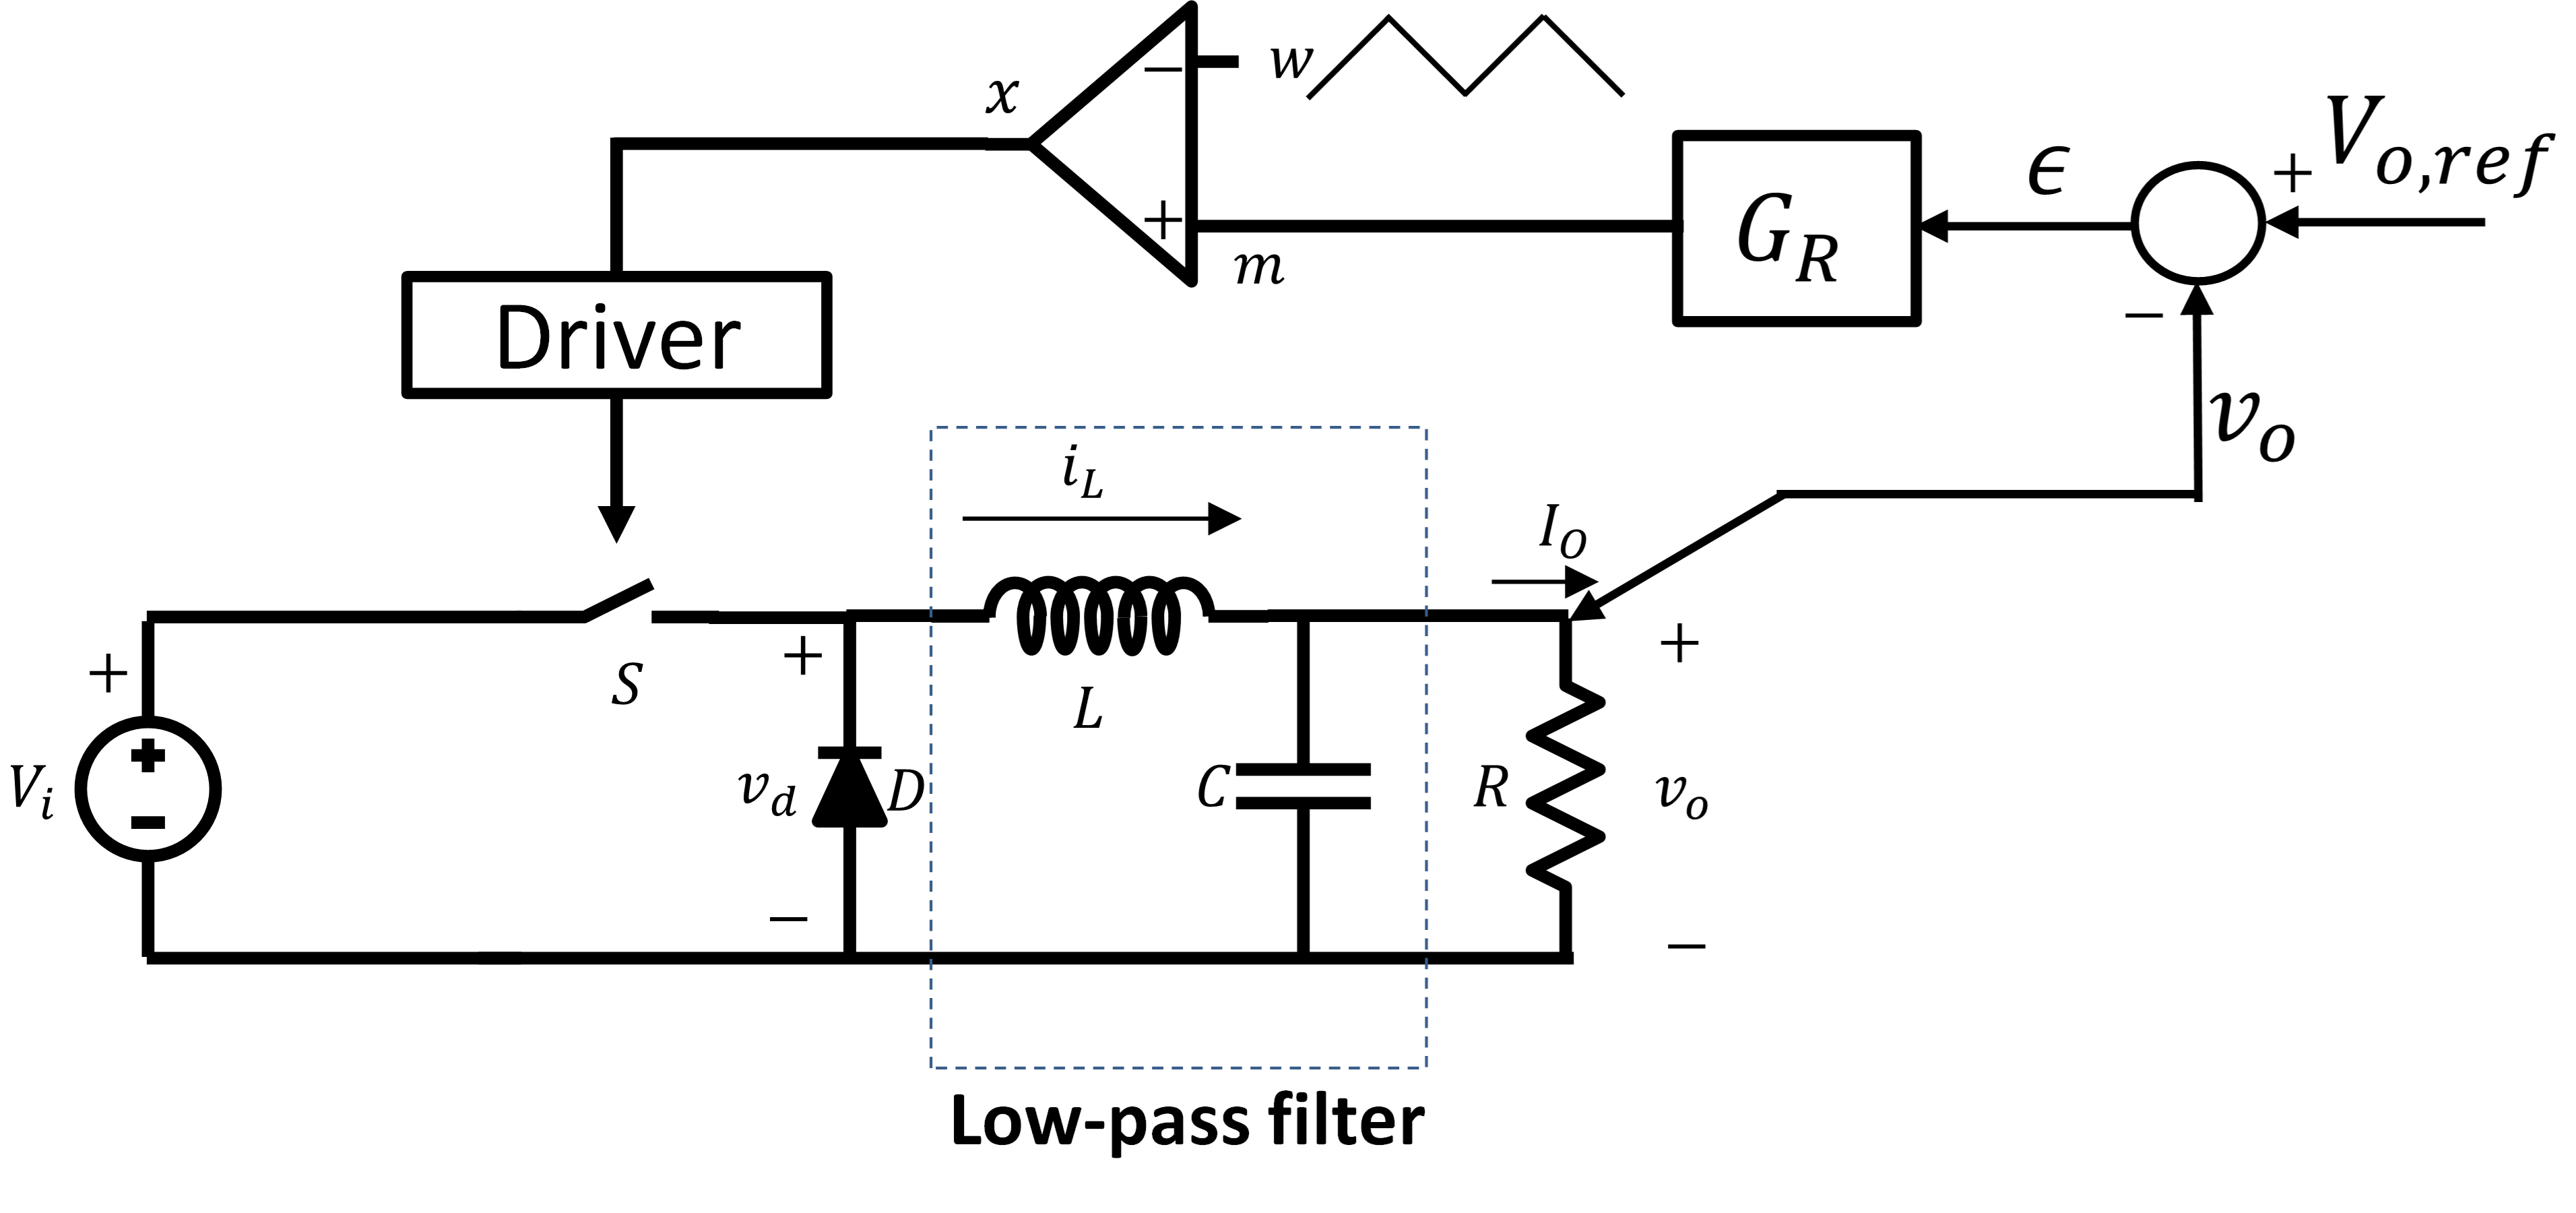
\includegraphics[width=0.8\linewidth]{images/Circuit2.png}
    \caption{Schema circuito}
    \label{fig:Circuit2}
\end{figure}
Il circuito è alimentato dalla tensione $V_i=+8V$,$V_{CC}=+8V$,$-V_{CC}=0V$ e utilizza il seguente range di tensione di riferimento $V_{o,ref}\in [0,+8]V$
\clearpage


\subsection{PRELAB}
\subsubsection{Dimensionamento del circuito}
\subsubsection{Diagramma di Bode del filtro RLC}
\begin{figure}[H]
    \centering
    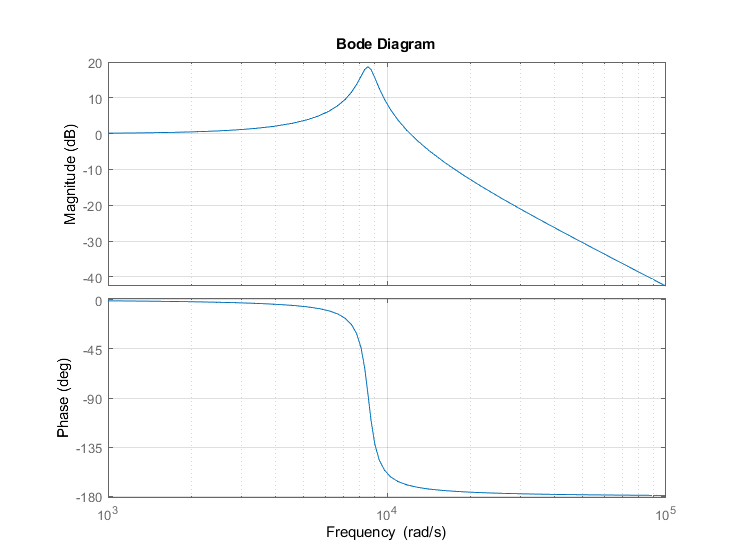
\includegraphics[width=0.6\linewidth]{images/Es2BodeRLC.png}
    \caption{Diagramma di Bode del filtro RLC}
    \label{fig:Es2BodeRLC}
\end{figure}
\subsubsection{Diagramma di Bode del circuito ad anello chiuso}
\begin{figure}[H]
    \centering
    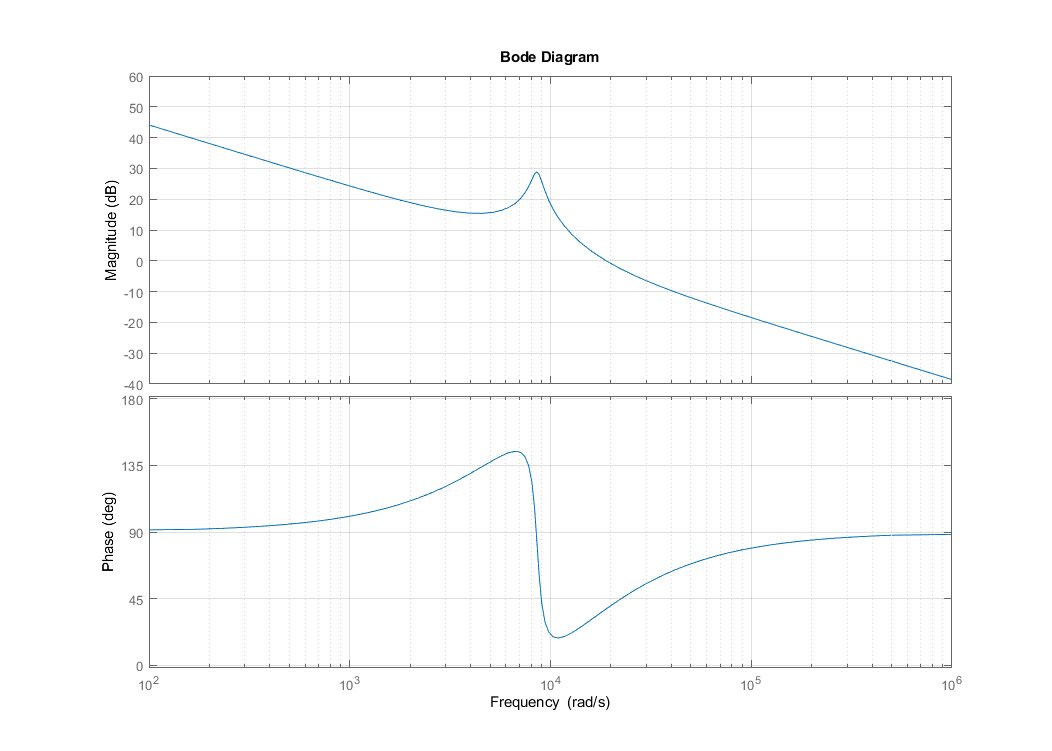
\includegraphics[width=0.6\linewidth]{images/Es2BodeCloseLoop.png}
    \caption{Diagramma di Bode del circuito ad anello chiuso}
    \label{fig:Es2BodeCloseLoop}
\end{figure}
\clearpage





\subsection{Assemblaggi e settaggi}
Dopo aver assemblato il circuito, seguendo lo schematico in Figura \ref{fig:Circuit2SPICE}. Abbiamo collegato un condensatore da $C=10\mu F$ in parallelo all'alimentazione OP amp (tra $+V_{CC}$ e $-V_{CC}$) in modo da ridurre in maniera più che apprezzabile i disturbi dell'amplificatore.
\begin{figure}[H]
    \centering
    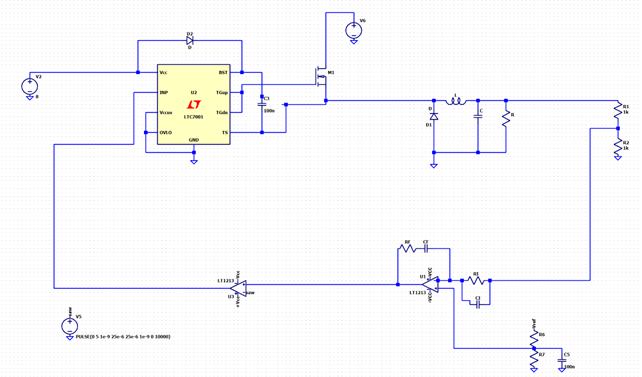
\includegraphics[width=0.9\linewidth]{images/Circuit2SPICE.png}
    \caption{Schematico SPICE del circuito}
    \label{fig:Circuit2SPICE}
\end{figure}
Tramite il generatore di funzioni abbiamo fornito al terminale invertente del secondo operazionale 1213 il seguente segnale:
\begin{itemize}
    \item Forma d'onda: triangolare
    \item Simmetria: 50\%
    \item Ampiezza: 5V picco-picco
    \item Tensione di offset: $V_{offset}=2.5V$
    \item Frequenza: $f=50kHz$
    \item Duty cycle: 50\%
\end{itemize}
Tale segnale viene usato dal comparatore operazionale per generare l'onda quadra per il gate driver LTC7001.
\clearpage






\subsection{Risultati}
Impostando la tensione di riferimento a $V_{ref}=4V$ abbiamo fatto delle misure dei segnali in vari punti del circuito, di cui riportiamo i relativi grafici dei segnali misurati:
\begin{itemize}
    \item In Figura \ref{fig:OutVoltage2} la tensione di uscita.
    \item In Figura \ref{fig:GateDriverINP} il segnale all'ingresso INP del gate driver LTC7001.
    \item In Figura \ref{fig:SawtoothSignal} il segnale onda triangolare simmetrica. 
    \item In Figura \ref{fig:CompareSawtoothINP} un confronto tra il segnale INP e l'onda triangolare.
    \item In Figura \ref{fig:U1Output} il segnale all'uscita del primo amplificatore U1.
\end{itemize}
\begin{figure}[H]
    \centering
    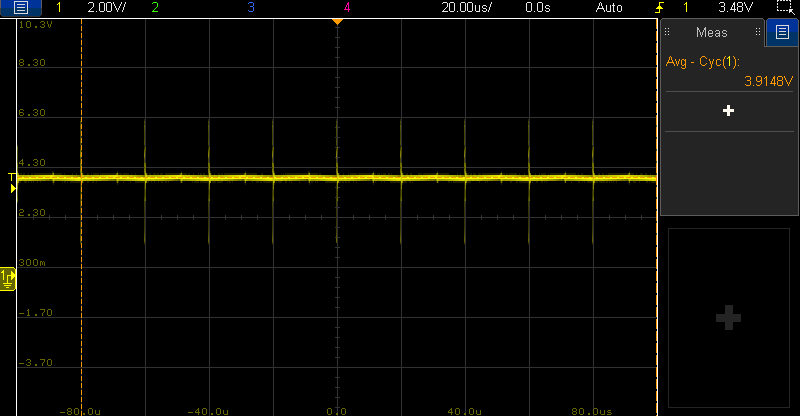
\includegraphics[width=0.6\linewidth]{images/scope_7.png}
    \caption{Tensione di uscita}
    \label{fig:OutVoltage2}
\end{figure}
\begin{figure}[H]
    \centering
    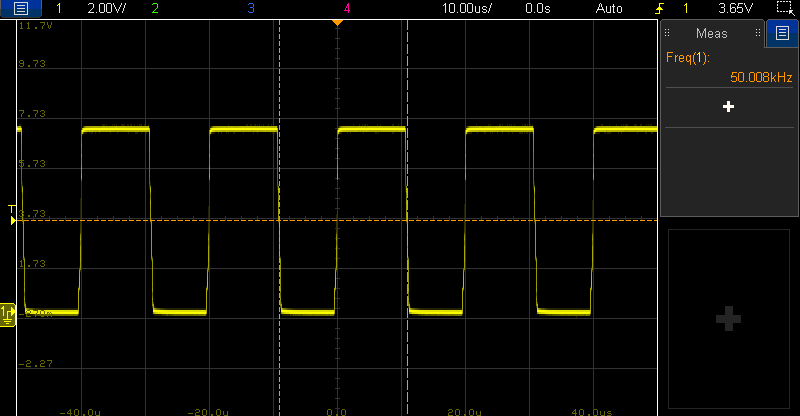
\includegraphics[width=0.6\linewidth]{images/scope_8.png}
    \caption{Segnale di ingresso al gate driver}
    \label{fig:GateDriverINP}
\end{figure}
\begin{figure}[H]
    \centering
    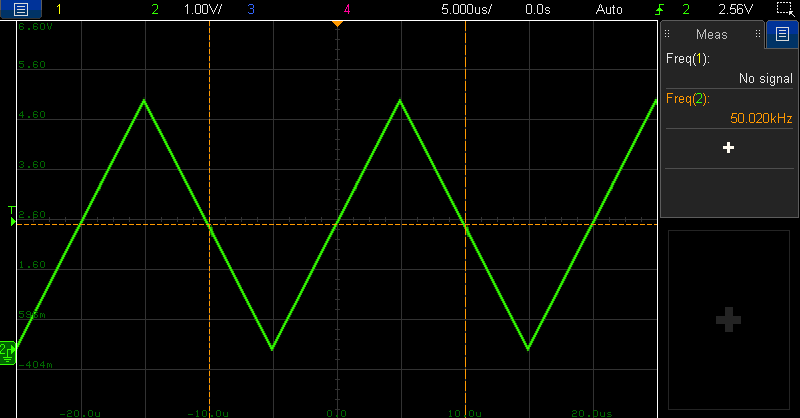
\includegraphics[width=0.6\linewidth]{images/scope_10.png}
    \caption{Segnale onda triangolare}
    \label{fig:SawtoothSignal}
\end{figure}
\begin{figure}[H]
    \centering
    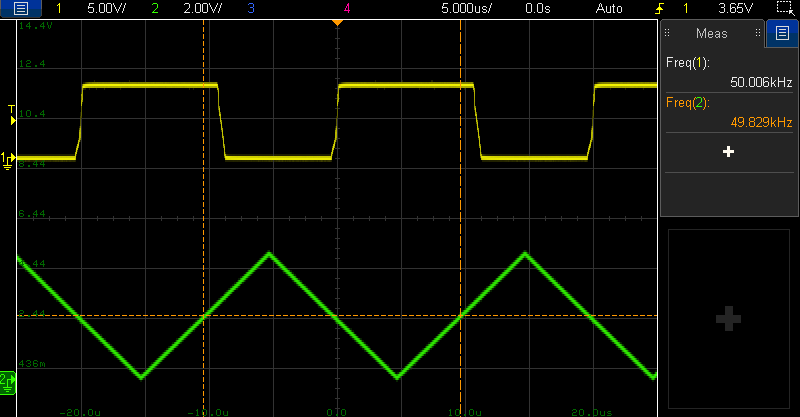
\includegraphics[width=0.6\linewidth]{images/scope_9.png}
    \caption{Segnale onda triangolare e segnale ingresso INP}
    \label{fig:CompareSawtoothINP}
\end{figure}
\begin{figure}[H]
    \centering
    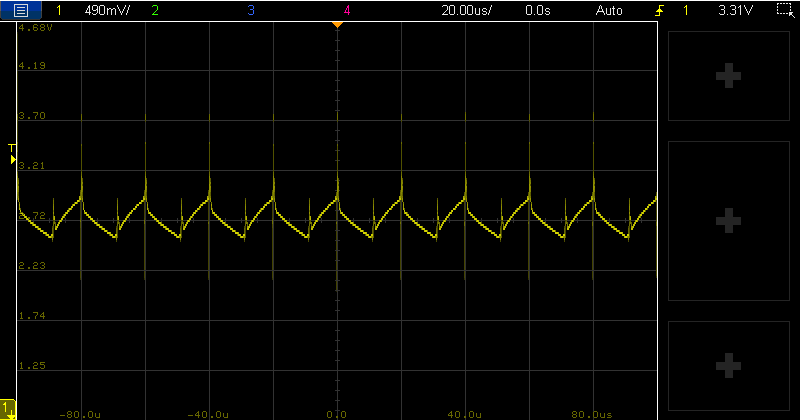
\includegraphics[width=0.6\linewidth]{images/scope_11.png}
    \caption{Segnale in corrispondenza dell'uscita di U1}
    \label{fig:U1Output}
\end{figure}
\clearpage
\subsubsection{Dipendenza tensione di uscita - $V_{ref}$}
In relazione alla tensione di riferimento impostata $V_{ref}$ abbiamo misurato la tensione di uscita $V_o$ e il duty cycle del segnale di ingresso al gate driver (pin INP). Abbiamo riportato le misure in Tabella \ref{tab:Tab2.3.1}
\begin{table}[H]
    \centering
    \begin{tabular}{|c|c|c|}
        \hline
        $V_{ref}(V)$&Duty cycle&$V_o(V)$\\\hline\hline
        $2.0V$&$30.49\%$&$1.9414V$\\\hline
        $2.5V$&$36.53\%$&$2.4433V$\\\hline
        $3.0V$&$42.68\%$&$2.9355V$\\\hline
        $3.5V$&$48.72\%$&$3.4372V$\\\hline
        $4.0V$&$54.76\%$&$3.9304V$\\\hline
        $4.5V$&$60.78\%$&$4.2222V$\\\hline
        $5.0V$&$66.80\%$&$4.9176V$\\\hline
        $5.5V$&$72.76\%$&$5.4018V$\\\hline
        $6.0V$&$78.77\%$&$5.9040V$\\\hline
    \end{tabular}
    \caption{Dati raccolti}
    \label{tab:Tab2.3.1}
\end{table}
Abbiamo poi successivamente plottato i risultati con MATLAB e abbiamo prodotto i seguenti grafici in Figura \ref{fig:Ris2TableVoVref} per quanto riguarda la relazione tra la tensione di uscita e il riferimento di tensione e in Figura \ref{fig:Ris2TableVrefDTC} la relazione tra duty cycle e riferimento di tensione.
\begin{figure}[H]
    \centering
    \begin{minipage}{.5\linewidth}
        \centering
        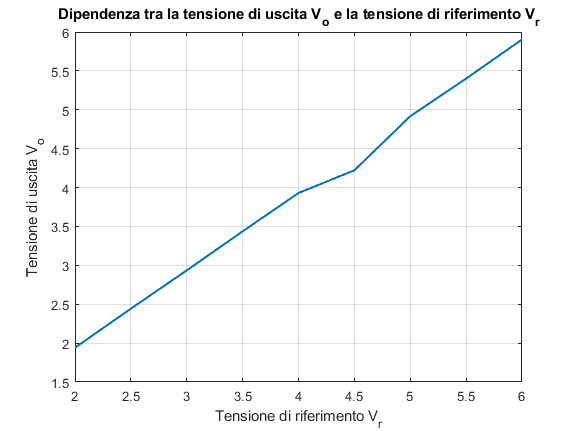
\includegraphics[width=\linewidth]{images/Ris2TableVoVref.png}
        \caption{}
        \label{fig:Ris2TableVoVref}
    \end{minipage}%
    \begin{minipage}{.5\linewidth}
        \centering
        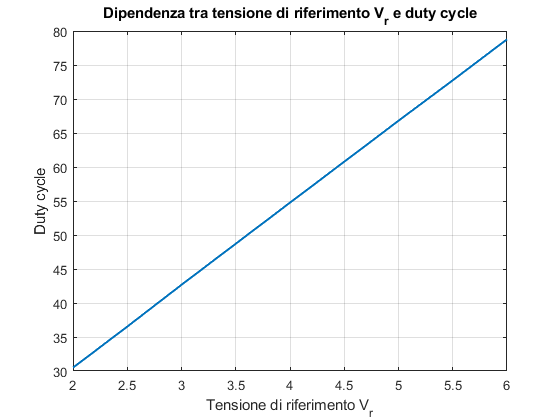
\includegraphics[width=\linewidth]{images/Ris2TableVrefDTC.png}
        \caption{}
        \label{fig:Ris2TableVrefDTC}
    \end{minipage}
\end{figure}
Notiamo dal grafico in Figura \ref{fig:Ris2TableVoVref} che la tensione, a parte per una leggera anomalia a 4.5V, ha andamento lineare. Dal grafico in Figura \ref{fig:Ris2TableVrefDTC} notiamo che l'andamento del duty cycle è perfettamente lineare. Questi due grafici confermano l'andamento teorico del nostro circuito.